\chapter{Technologia CUDA}
\section{Współbieżna przyszłość}
Kiedy w roku 2005 Herb Sutter \cite{lunch} opublikował artykuł o intrygująco 
brzmiącej nazwie 'Koniec darmowego lanczu', w szeroko pojętym środowisku 
deweloperskim rozgorzała dyskusja. Autor stwierdził, że obserwujemy kres 
wykładniczego wzrostu wydajności mikroprocesorów, rozumianego przez wzrost 
częstotliwości taktowania ich zegarów w zależności od ilości użytych
tranzystorów. Z tym argumentem, nie można się nie zgodzić patrząc na
oferowane na rynku procesory firmy Intel przedstawione na rysunku \ref{proce}.

\begin{figure}[ht]
\centering
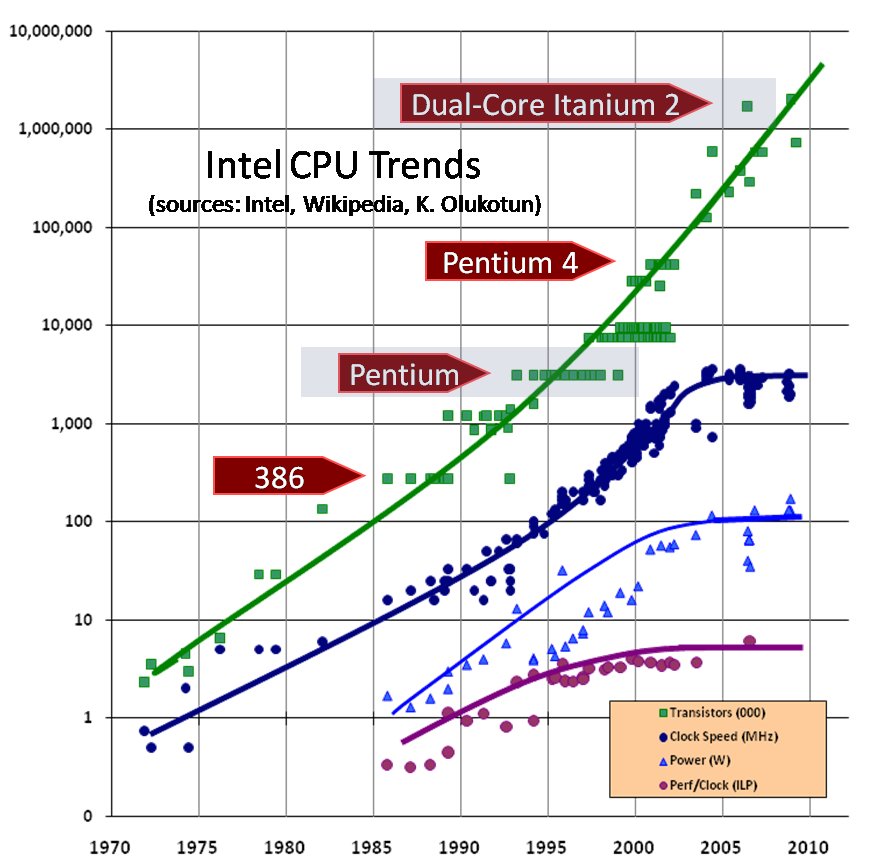
\includegraphics[scale=1.0]{images/CPU.png}
\caption{Charakterystyki procesorów firmy Intel na przestrzeni 40 lat. Źródło: http://www.gotw.ca/}
\label{proce}
\end{figure}

Ważniejszą jednak tezą postawioną przez Suttera było stwierdzenie, że
programiści nie będą mogli dłużej korzystać ze wzrostu mocy obliczeniowej
sprzętu. Taki wzrost wydajności często okazywał się dla twórców aplikacji
niezastąpiony. Napotykając problemy wydajnościowe w swoim oprogramowania
programiści mogli albo poświęcić się żmudnemu procesowi optymalizacji, albo
po prostu podnieść jej wymaganie sprzętowe. Często, głównie ze względów
ekonomicznych drugi wariant było wybierany, gdyż ograniczał się do tylko do
poczekania na nowe generacje sprzętu. To zjawisko, ciekawie scharakteryzował J.
Spolsky przytaczany w \cite{nolunch} ,,Jako programista masz wybór, albo
spędzisz pół roku na przedesignowaniu swojej aplikacji, wstawiając kod asemblera
w krytycznych sekcjach, albo na wakacjach, grając na perkusji w rockowej kapeli.
Niezależnie od alternatywy którą wybierzesz, twoja aplikacji będzie działała
szybciej,,.

Czy jednak założenie o niskim wzroście wydajności współczesnym mikroprocesorów
jest prawdziwe? Wprawdzie częstotliwość taktowania nie podlega już takim trendom
co wcześniej, jednak dzisiejsze architektury CPU oferują więcej niż jeden rdzeń
zdolny do wykonywania programu. Obecnie na rynku jest już oferowany procesor
Intel z serii i7, który może posiadać do 8 fizycznych rdzeni. Dodatkowo, nowe
technologie takie jak hyperthreading, pipelining czy zaawansowane branch
prediction pozwalają na możliwie szybkie, czy wręcz równoległe wykonywanie
fragmentów sekwencyjnego kodu.

Mimo nowoczesnej architektury CPU, sekwencyjnie programy i tak wykonywane są
tylko na pojedynczym rdzeniu\cite{massive}, który jak było to opisane wcześniej,
na przestrzeni ostatnich lat stał się znacząco szybszy. Nawet 
procesory posiadające instrukcje typu SIMD oraz heurystyki wykorzystywane w
nowoczesnych kompilatorach, takie jak np. 'Loop Vectorizer' wykorzystywany w
kompilatorach bazujących na LLVM \cite{llvm} czy 'Auto-Vectorization' w GCC
\cite{gcc} nie są w stanie zamienić sekwencyjnego kodu w wydajny kod
współbieżny.

Sutter stwierdza, że odpowiedzą na postawiony wyżej problem jest zmiana
paradygmatu z programowania sekwencyjnego na współbieżne. Tworzone wielowątkowe
aplikacje będą w stanie korzystać z wielordzeniowych architektur, co przyspieszy
ich wykonywanie a programistom pozwoli nadal oczekiwać na ,,darmowy lancz''.
Faktem potwierdzającym postawioną przez niego tezę jest rysunek \ref{gflops},
przedstawiający teoretyczną maksymalną wydajność wielo-rdzeniowych mikroprocesorów oraz układów
graficznych mierzoną w giga FLOPS-ach (operacji zmiennoprzecinkowych na
sekundę).

\begin{figure}[ht]
\centering
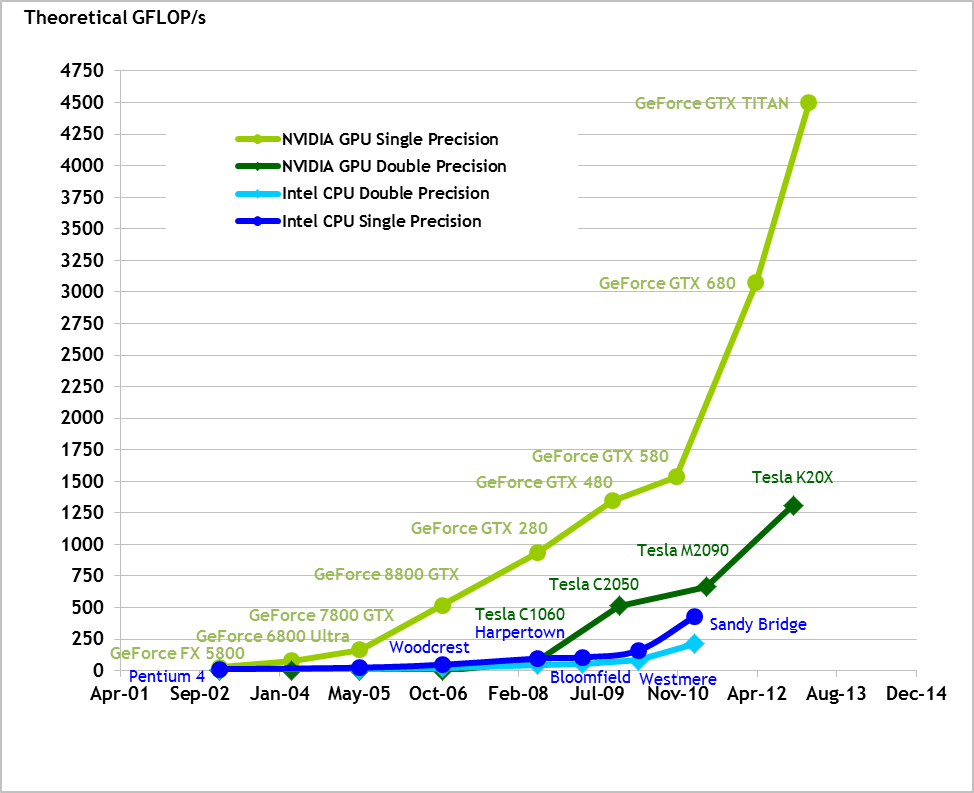
\includegraphics[scale=0.4]{images/floating-point-operations-per-second.png}
\caption{Teoretyczna wydajność mierzona w GFLOP/s w czasie. Źródło: CUDA C Programming Guide}
\label{gflops}
\end{figure}

Samo jednak przejście na model programowania równoległego nie będzie łatwe,
przyjemne, a przede wszystkim tanie. Wg
Suttera taka zmiana wiązać się będzie nie tylko ze zmianą architektury
aplikacji czy konstrukcjami języków programowania. 

Zmiany w stronę wielowątkowości obserwowane są od jakiegoś czasu. Dla przykładu
w 
standardzie języka C++ 11, biblioteka obsługująca wątki wchodzi w skład
biblioteki standardowej, Microsoft publikuje bibliotekę C++ AMP i wielowątkowe
wersje popularnych bibliotek dla Platformy .NET jak PLINQ, a NVIDIA biblioteki
algorytmiczne m.in. CUFFT wykonywane na GPU. Marsz w stronę wielowątkowości
obserwujemy cały czas, ale moim zdaniem nie będzie to jednak rewolucja
zapowiadana w \cite{rewolucja}, lecz bardziej ewolucja. Warto dodać, że dużo
pracy zostało już wykonane.  Serwery www oraz bazy danych są świetnym przykładem
dobrze skalowanych, wielowątkowych aplikacji.

Kolejną istotną kwestią w projektowaniu wielowątkowych aplikacji jest jej
skalowalność. Jeżeli dany problem programistyczny nie może być
dynamicznie dzielony na podproblemy, które będą mogły być rozwiązane
indywidualnie, korzyści związane z przyrostem ilości rdzeni w sprzęcie nie będą
zauważalne. Taki podział często okazuje się być nietrywialny, a czasem
wręcz niemożliwy. Nie można też oczekiwać wzrostów wydajności równych ilości
zrzenia, ponieważ nie
cały kod aplikacji może być zrównoleglony. Dobrze opisuje to formuła stworzona w
1967 r. przez G. Amdahla:

\begin{equation}
W(N) = \frac{1}{(1-S) + \frac{S}{N}},
\end{equation}
gdzie $N$ jest ilością jednostek wykonywania, a $S$ jest częścią kodu programu,
	który może być zrównoleglony. I tak dla 8 rdzeni i programu o współczynniku
	$S=60\%$, otrzymujemy wzrost wydajności tylko około 2.1 raza.

Zakładając hipotetycznie, że mamy do dyspozycji nieograniczoną liczbę jednostek
wykonania, czyli $n \to \infty$ to maksymalny wzrost wydajności
wg Amdahla wynosić będzie tylko 2.5 raza.
Współbieżność jest bez wątpienia problemem z którym każdemu programiście
przyjdzie się kiedyś zmierzyć. Możliwe, że do niektórych problemów wystarczą mu
gotowe rozwiązania z dostępnych bibliotek, jednak myślenie o problemie i
przedstawienie go w postaci dającej się zrównoleglić będzie rzeczą
najważniejszą. Środowiska naukowe pomagają w tym aspekcie bardzo istotnie.
Każdego roku publikowane są artykuły przedstawiające często nowatorskie
podejścia do standardowych problemów, wskazując możliwość ich współbieżnego rozwiązania.
Przewiduję, że w następnych latach trend z programowaniem równoległym będzie
przybierał na sile, czego owocem będą nowe, innowacyjne metody i technologie.

\section{Powstanie CUDA}

Technologia CUDA (Compute Unified Device Architecture) została po raz pierwszy
zaprezentowana przez NVIDIA w listopadzie 2006 r. Związana jest ona z nowym
modelem
programowania aplikacji w którym sekwencyjne fragmenty kodu są wykonywane na
CPU, natomiast te wymagające obliczeniowo, na procesorach graficznych (GPU).
Pierwsze karty graficzne z serii GeForce 8800, implementujące technologię CUDA,
		 pojawiły się w roku 2006 r. Programiści od tego czasu mogą korzystać ze
		 specjalnie zaprojektowanych w tym celów interfejsów programistycznych
		 bibliotek CUDA.

Sama koncepcja programowania procesorów graficznych jest znana od dawna.
Programiści używając interfejsów do programowania shaderów, dostępnych chociażby
w OpenGL 1.4 (2002) czy Direct3D 8.0 (2001), mogli dokonywać 
obliczeń na kartach graficznych. Wymagało to jednak często wielu trików, takich
jak przekazywanie danych poprzez tekstury czy odczytywania danych wyjściowych z
wygenerowanej ramki obrazu. NVIDIA wyszła naprzeciw tym problemom, tworząc
dedykowane do tego interfejsy programistyczne w języku C.

Na sukces technologi CUDA złożyło się wg \cite{massive} parę czynników.
Pierwszym jest fakt, że programiści aplikacji równoległych otrzymali środowisko
w którym ich kod, wg zapewnień NVIDIA, będzie wykonywany poprawnie, niezależnie
od używanego sprzętu. Ma to szczególnie ważne znaczenie, biorąc pod uwagę fakt,
   że projektanci kart graficznych nie zakładali początkowo ich użycia do
   obliczeń inżynierskich. I tak np. kalkulacje na liczbach zmiennoprzecinkowych
   na różnych kartach graficznych NVIDIA do 2006 r. mogły skutkować nieznacznie innymi
   wynikami. Dopiero specyfikacja technologii CUDA wymusiła na projektantach
   sprzętu zgodność ze standardami publikowanymi przez IEEE.

Kolejnym czynnikiem, który zdecydował o sukcesie technologii CUDA jest
dostępność medium, na którym wielowątkowe, zrównoleglone aplikacje mogą być
wykonywane. W chwili obecnej na rynku znajdują się setki milionów kart
graficznych wyprodukowanych przez NVIDIA zdolnych do wykonania kodu napisanego w
CUDA. Ma to bardzo istotny wymiar ekonomiczny, ponieważ wiele specjalistycznych
(np. w medycynie) aplikacji nie musi być dostarczana wraz z drogim,
	dedykowanym dla tego celu sprzętem. Spowodowało to zatem wzrost rynku dla
	tego typu rozwiązań i stworzyło ekonomiczne uzasadnienie do dalszej pracy
	nad współbieżnie wykonywanymi aplikacjami.

Istotne było też zwiększenie dokładności dokonywanych obliczeń na kartach
graficznych poprzez umożliwienie użycia liczb podwójnej precyzji. Obecnie
wszystkie karty NVIDIA , począwszy od architektury Fermi, pozwalają na
korzystanie z liczb zmiennoprzecinkowych o zwiększonej precyzji.

Ostatnim, najbardziej oczywistym czynnikiem, jest wzrost wydajności. Procesory
graficzne składające się z multiprocesorów strumieniowych są przystosowane do
przetwarzania dużej ilości danych jednocześnie. Dodatkowo narzut związany z
kreacją i zarządzaniem pojedynczego wątku na GPU jest znacząco mniejszy niż
analogiczna operacja wykonana na CPU.  W nowych architekturach takich jak
GeForce z serii 780 posiadających aż 2304 rdzenie zdolne do równoległego
wykonywania kodu. Efektem jest wzrost wydajności aplikacji średnio
o 2.5 raza \cite{cpuvsgpu}.

\section{Interfejs programisty}

\subsection{Kompilacja}

Zaproponowany we frameworku CUDA model programowania zakłada możliwość
skompilowania i wykonywania kodu programu w dwóch różnych kontekstach -
gospodarza (CPU) oraz GPU (procesora graficznego)\cite{Nvi11b}. Jako kontekst rozumiany jest
specyficzny dla danej architektury zestaw instrukcji dla procesora. Fragmenty
programu, których zrównoleglenie jest niemożliwe są tworzone w kontekście
gospodarza,
	natomiast te wymagające intensywnych, wielowątkowych obliczeń w kontekście
	GPU.  Współistnienie dwóch kontekstów w jednym programie wykonywalnym
	możliwe jest dzięki zestawie bibliotek i narzędzi dostarczanych wraz z
	pakietem CUDA.

Biblioteki dostarczane wraz z pakietem CUDA umożliwiają pisanie kodu CUDA w różnych
językach programowania. Najczęściej stosowanych jest język C, istnieją jednak biblioteki
dla języków C++, Java, Python czy Fortran. Dodatkowo kod CUDA może być też pisany w specjalnie stworzonym do tego celu
niskopoziomowym języku PTX (Pararell Thread Execution), przypominającym
asembler
Cechą wyróżniającą kod PTX od skompilowanego kodu binarnego, jest możliwość jego
kompilacji w locie z użyciem tzw. kompilatora JIT (ptxas) dostarczanego przez
NVIDIĘ wraz ze sterownikami do karty graficznej. Pozwala to na uruchamianie kodu
CUDA nie tylko na różnych wersjach sterowników karty graficznej, lecz również na
innych procesorach graficznych firmy NVIDIA bez potrzeby rekompilacji\cite{isa}.

\begin{figure}[ht]
\centering
\tikzstyle{layer}=[rounded corners=10pt,shading=center]

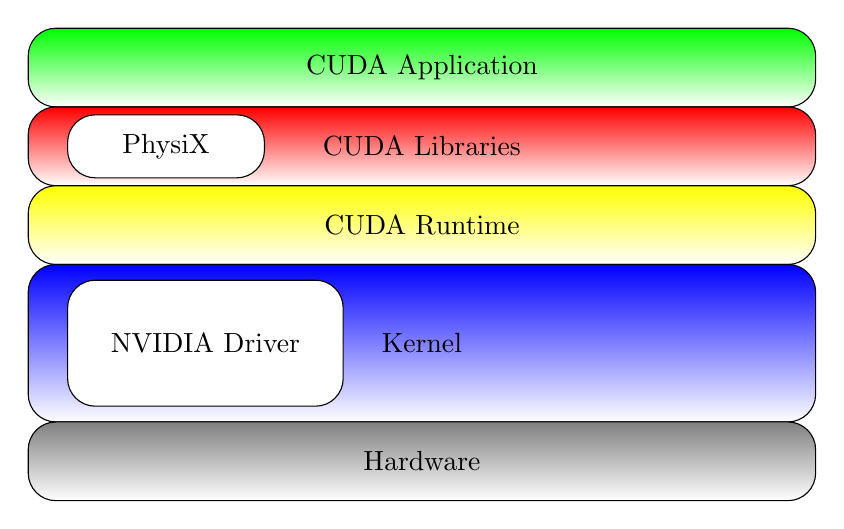
\begin{tikzpicture}
\draw[style=layer,top color=green] (0,0) rectangle (10,1) node[pos=0.5] {CUDA Application};
\draw[style=layer,top color=red] (0,-1) rectangle (10,0) node[pos=0.5] {CUDA
	Libraries};
\draw[style=layer,top color=white] (0.5,-0.9) rectangle (3,-0.1) node[pos=0.5]
{PhysiX};
\draw[style=layer,top color=yellow] (0,-2) rectangle (10,-1) node[pos=0.5] {CUDA
	Runtime};
\draw[style=layer,top color=blue] (0,-4) rectangle (10,-2) node[pos=0.5] {Kernel};
\draw[style=layer,top color=white] (0.5,-3.8) rectangle (4,-2.2) node[pos=0.5]{NVIDIA Driver};
\draw[style=layer,top color=gray] (0.0,-5) rectangle (10,-4) node[pos=0.5]{Hardware};

\end{tikzpicture}

\caption{Stos CUDA. Źródło: Opracowanie własne.}
\label{cuda-model}
\end{figure}

CUDA to w rzeczywistości cały stos bibliotek, sterowników i narzędzi. Jest on
ogólnie 
przedstawiony na rysunku \ref{cuda-model}. Najważniejszymi elementami w całym
stosie jest sterownik dostarczany przez producenta karty graficznej
oraz biblioteka CUDA Runtime (cudart). Zadaniem sterownika, uruchomionego
jako moduł jądra systemu operacyjnego, jest dostęp do urządzenia oraz wykonanie
na nim kodu dedykowanego dla jego architektury i wersji. Sterownik odpowiada za
komunikację z urządzeniem a biblioteka CUDA Runtime nadbudowuje nad nim wyżej
poziomowe funkcje takie jak inicjalizacja, wywołanie kontekstu GPU czy
kopiowanie danych między kartą a pamięcią RAM komputera.

Niezależnie od wybranego języka programowania czy użytych bibliotek, ostatecznie kod programu CUDA musi
zostać skompilowany do postaci binarnej i uruchomiony w kontekście gospodarza. W
czasie działania programu wykonywanego sekwencyjnie na CPU, następuje zmiana
kontekstów i uruchomienie skompilowanych fragmentów kodu na procesorze graficznym.
Przełączanie kontekstów jest transparentne dla programisty,
ponieważ ogranicza się tylko do wywołania odpowiednich funkcji z bibliotek
dostarczanych wraz z pakietem CUDA.

CUDA to nie tylko zestaw bibliotek, lecz również zestaw rozszerzeń do języka
programowania C. Implementacja rozszerzeń podytkowana była potrzebą
jednoznacznego rozróżnienia fragmentów programu każdego z kontekstów w kodzie
źródłowym. W rezultacie można pisać kod CUDA używając ANSI C
oraz specjalnych rozszerzeń przypominających atrybuty kompilatora. W ten sposób
NVIDIA zaoszczędziła programistom CUDA potrzeby nauki nowego języka
programowania, czy pisania kodu w niskopoziomowym języku PTX. Użycie
specjalistycznych atrybutów kompilacji dla języka C, możliwe jest tylko dzięki
wykorzystaniu dostarczanego wraz z frameworkiem CUDA kompilatora 'nvcc'.

NVIDIA Cuda Compiler (nvcc) nie jest kompilatorem w tradycyjnym tego słowa
znaczeniu, a bardziej zestawem narzędzi służących do kompilacji. W przypadku gdy
kod źródłowy będzie kompilowany tylko w kontekście gospodarza, właściwą kompilacją
zajmują się kompilatory dedykowane dla danego systemu operacyjnego. Dla
Windows nvcc wykorzystuje kompilator Visual Studio, natomiast dla systemu Linux
użyty jest m.in. GCC. Zadaniem NVCC jest ukrycie przed programistą etapów kompilacji
specyficznego kodu CUDA przeznaczonego do wykonania na procesorze
graficznym. Schemat kompilacji wraz z poszczególnymi etapami przedstawia rysunek
\ref{compilation}.

\begin{figure}[H]
\centering
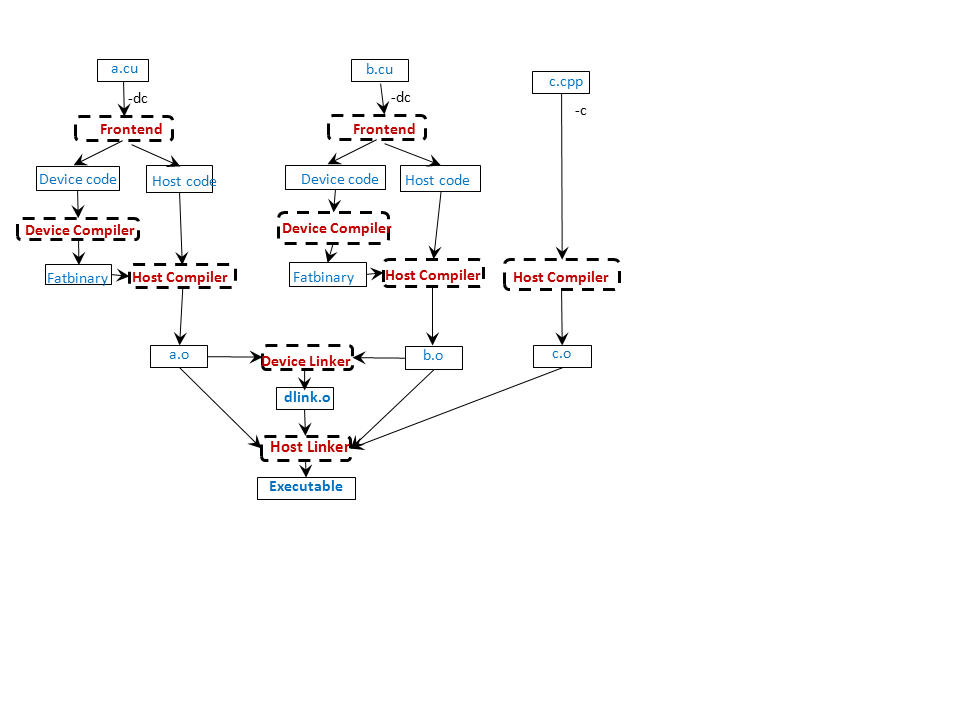
\includegraphics[scale=0.8]{images/nvcc-options-for-separate-compilation.png}
\caption{Schemat rozłącznej kompilacji przy użyciu NVCC. Źródło: CUDA Compiler Driver NVCC}
\label{compilation}
\end{figure}

Pliki źródłowe programu napisanego w języku C zawierające rozszerzenia CUDA, przyjęło się zwyczajowo
oznaczać przyrostkiem ".cu", aby odróżnić je od konwencjonalnych programów C
oznaczanych przyrostkiem ".c". Oba rodzaje rozszerzeń są akceptowane przez NVCC, co
pozwala na wykorzystanie do kompilacji projektów CUDA tylko jednego kompilatora.
W celu ułatwienia procesu budowania NVCC wspiera większość tradycyjnych
parametrów kompilatora znanych z GCC czy Visual Studio Compiler. 

NVCC używane jest zazwyczaj do kompilacji kodu źródłowego do postaci binarnej.
Możliwe jest także użycie kompilatora do kompilacji kodu napisanego w C do
postaci pośrednich takich jak PTX, fatbin czy cubin. Fatbin jest plikiem
zawierającym kod PTX w wersjach dla różnych architektur kart graficznych.  W
momencie kompilacji w locie (JIT) sterownik karty graficznej potrafi z pliku
fatbin wybrać ten kod PTX, który najlepiej odpowiada jego wersji i modelowi
karty graficznej. Skutkuje to wyborem zoptymalizowanego dla danej architektury
kodu oraz skróceniem czasem ładowania aplikacji. Natomiast Cubin jest to plik
binarny przeznaczony dla konkretnego procesora graficznego, który nie jest
kompatybilny z innymi architekturami procesorów graficznych.

\subsection{Kernele}
Z punktu widzenia programisty wykonanie fragmentu kodu w kontekście GPU
ogranicza się do wywołania specyficznego rodzaju funkcji, nazywanego w nomenklaturze CUDA kernelami.
Kernele w języku C oznaczone są specjalnym atrybutem kompilatora
\texttt{\_\_global\_\_} oraz mają
specyficzną konwencję wywołania przedstawioną na listingu \ref{kernel}.

Funkcja kernela wykonywana jest na procesorze graficznym jednocześnie przez $M$
różnych wątków. W celu określenia dokładnej ilości wątków dla których ma się ona
wykonać oraz sposobu ich indeksowania, dwa dodatkowe parametry
są przekazane do funkcji kernela między znacznikami $<<<$ oraz $>>>$. Pierwszy parametr
oznacza liczbę tzw. bloków, czyli 1, 2 lub 3 - wymiarowych grup ograniczających
wątki. Drugi parametr to wymiar pojedynczego bloku, określany jako pojedyncza liczba
całkowita lub specjalnym typ $dim3$, służący do określenia rozmiarów 2 lub
3-wymiarowego bloku. Po zdefiniowaniu ilości i wielkości bloków indeksy wątków dostępne
są w ciele funkcji dzięki predefiniowanej zmiennej $threadIdx$.

\begin{lstlisting}[caption=Dodawanie macierzy, label=kernel]
// Definicja funkcji kernela
__global__ void MatAdd(float A[N][N], float B[N][N],
		float C[N][N])
{
	int i = blockIdx.x * blockDim.x + threadIdx.x;
	int j = blockIdx.y * blockDim.y + threadIdx.y;
	if (i < N && j < N)
		C[i][j] = A[i][j] + B[i][j];
}

int main()
{
	...
	// Wywolanie kernela CUDA na bloku o wymiarach 16x16
	dim3 threadsPerBlock(16, 16);
	dim3 numBlocks(N / threadsPerBlock.x, N / threadsPerBlock.y);
	MatAdd<<<numBlocks, threadsPerBlock>>>(A, B, C);
	...
}
\end{lstlisting}

Grupę bloków zleconą do wykonania z użyciem CUDA nazywa się siatką
(ang. grid). Ogólny schemat siatki przedstawia rysunek \ref{grid}. Podobnie jak
wątki, bloki mogą być indeksowane jedno lub dwuwymiarowo. Ich indeksy są dostępne
w funkcji kernela pod specjalną zmienną $blockIdx$, natomiast rozmiar samego
bloku możliwy jest do pobrania poprzez zmienną $blockDim$.

\begin{figure}[H]
\centering
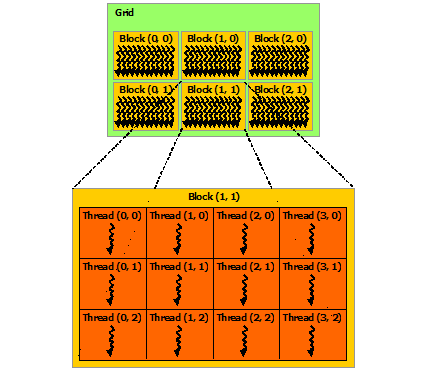
\includegraphics[scale=0.8]{images/grid-of-thread-blocks.png}
\caption{Źródło: CUDA Programming Guide}
\label{grid}
\end{figure}

Specyfikacja CUDA gwarantuje, że pojedynczy blok wykonywany jest na
dokładnie jednym procesorze graficznym. W efekcie, wątki wchodzące w
skład danego bloku wykonywane są sprzętowo współbieżnie. Same bloki zaś w zależności od
możliwości obliczeniowych urządzenia wykonywane są również
współbieżnie na procesorze graficznym lub w przypadku braku zasobów -
sekwencyjnie, czyli dopiero po
zakończeniu wykonywania poprzedzającego bloku. Taki model programowania zapewnia
skalowalność rozwiązania w przypadku posiadania przez urządzenie więcej niż
jednego procesora graficznego oraz pozwala programiście skupić się na
optymalizacji wykonania programu w ramach pojedynczego bloku, zostawiając frameworkowi CUDA
zadanie optymalnej alokacji bloków między dostępne procesory.
 Programy pisane w CUDA muszą więc uwzględniać fakt,
że bloki mogę być wykonywane w dowolnej kolejności. 


\begin{lstlisting}[caption=Funkcje CUDA, label=cudafunc]
// Definicja funkcji
__device__ float square(float a)
{
	return a * a;
}
\end{lstlisting}

Definicja kernela nie jest jedynym rozszerzeniem języka C dostępnym w
kompilatorze NVCC. Możliwa jest również definicja funkcji wykonywanej w
kontekście GPU poprzez oznaczenie jej atrybutem \texttt{\_\_device\_\_} (listing
		\ref{cudafunc}). Tak zdefiniowana funkcja może być użyta w funkcji
kernela, pozwalając na enkapsulację często powtarzanych fragmentów kodu. Należy
jednak pamiętać, że kontekst gospodarza i GPU znacząco się od siebie różnią i w
przypadku tego drugiego wywołania funkcji z reguły trwają dużo
dłużej\cite{Nvi11b} Kompilator NVCC na ogół stara się więc inlajnować wszystkie
funkcje oznaczone atrybutem \texttt{\_\_device\_\_}, czyli umieszcza ich kod
bezpośrednio w miejscu wywołania. Wydłuża to docelowy kod kernela, jednak
znacząco przyspiesza jego wykonywanie. W celu wymuszenia na kompilatorze braku
inlajnowania trzeba poprzedzić atrybut \texttt{\_\_device\_\_} atrybutem
\texttt{\_\_noinline\_\_}, natomiast w celu zagwarantowania inlajnowania funkcji
atrybutem \texttt{\_\_forceinline\_\_}.

\subsection{Hierarchia pamięci}
\label{ssec:mem}

W modelu CUDA wyróżnia się 4 podstawowe typy pamięci:
\begin{itemize}
\item Rejestry
\item Pamięć Dzielona (Shared Memory)
\item Pamięć Stała (Const Memory)
\item Pamięć Globalna
\end{itemize}

Rejestry ogólnego przeznaczenia procesora graficznego są najszybszym rodzajem
pamięci dostępnej na GPU.  Ich ilość jest jednak mocno ograniczona, dlatego
programista CUDA musi poświęcić szczególną uwagę aby zapewnić możliwe dobre ich
wykorzystanie. Rejestry są najczęściej alokowane w przypadku tworzenia i
używania zmiennych tymczasowych. Dostęp do zmiennych lokalnie zdefiniowanych
możliwy jest tylko z jednego wątku, dlatego w celu wymiany informacji pomiędzy
wątkami zachodzi potrzeba użycia innego rodzaju pamięci.

Pamięć dzielona to szybka pamięć L1 służąca do wymiany danych między wątkami.
Ponieważ cache L1 jest dostępny tylko dla danego procesora graficznego,
  pamięć ta może być współużytkowana tylko w ramach pojedynczego bloku. W celu
  deklaracji pamięci dzielonej NVCC wprowadza nowy atrybut o nazwie
  \texttt{\_\_shared\_\_}. Odwołania do pamięci dzielonej zajmuje parę razy
  więcej cykli zegara niż odwołanie do rejestru, jednak i tak liczba ta jest
  znacząco mniejsza od cykli potrzebnych do pobrania danych z pamięci globalnej.
  Wielkość pamięci dzielonej dostępnej na procesorze jest niewielka i dla
  architektury Kepler wynosi 48 KB.

Pamięć stała to w istocie pamięć L1 stworzona i używana do renderowania tekstur 
w grafice komputerowej. Powodem zastosowania tej pamięci jest zmniejszenie czasu
dostępu do danych mieszczących się w pamięci globalnej, których nie modyfikuje się w trakcie działania programu.
W tym celu użyty jest dodatkowy cache L1, który przechowuje kopię danych 
z pamięci globalnej i dostępny jest tylko w trybie do odczytu.
Aby zadeklarować zmienną tego typu, która może zostać odczytana z dowolnego
wątku lub bloku używa się atrybutu \texttt{\_\_constant\_\_}.

Ostatnim rodzajem pamięci wykorzystywanej w modelu CUDA jest pamięć globalna.
Jest to pamięć typu DRAM o znacznej pojemności, wynoszącej w chwili pisania tej
pracy, nawet do 4 GB w najbardziej zaawansowanych kartach dostępnych na rynku. 
Wadą jej jest natomiast bardzo długi czas dostępu.

Schemat wątków i bloków z przypisaniem poszczególnych rodzajów pamięci, do których
mają dostęp podsumowują rysunki \ref{hier} oraz \ref{hier2}.

\begin{figure}[H]
\centering
\label{hier}
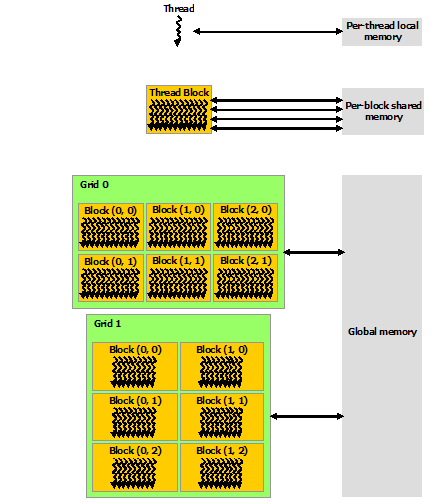
\includegraphics[scale=0.5]{images/memory-hierarchy.png}
\caption{Dostęp do pamięci w modelu CUDA. Źródło: \cite{Nvi11b}}
\end{figure}

\begin{figure}[H]
\centering
\label{hier2}
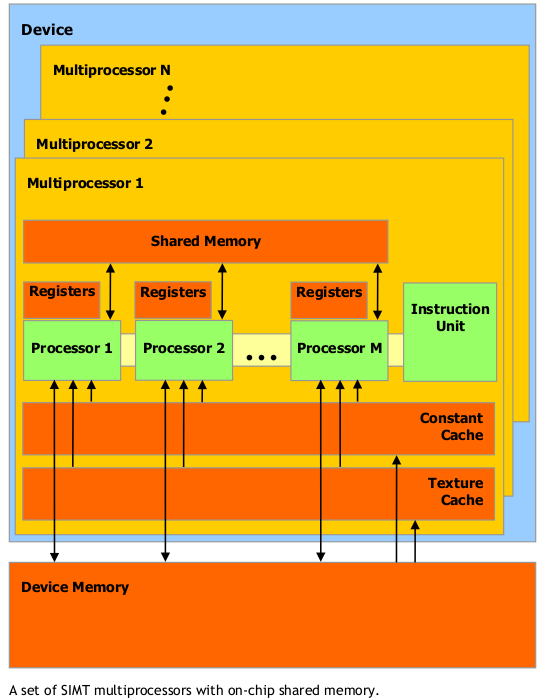
\includegraphics[scale=0.6]{images/gpu.png}
\caption{Dostęp do pamięci w modelu CUDA. Źródło: \cite{Nvi11b}}
\end{figure}

\section{GPU}
\subsection{Procesor graficzny}
W rozdziale tym przedstawiona zostanie architektura procesora graficznego na
przykładzie modelu Geforce GTX 680. Wykonany jest on w architekturze Kepler
wprowadzonej przez NVIDIA w 2012 r. Nie jest to najnowsza architektura stworzona
dotąd przez NVIDIA, jednak wybór ten jest podyktowany dwoma
względami. Pierwszą prozaiczną przyczyną jest fakt, że autor tej pracy posiada
do dyspozycji model 660M wykonany w tej samej architekturze, a drugim że
dostępne są materiały, opublikowane przez NVIDIA, omawiające architekturę Kepler
na przykładzie Geforce GTX 680.

Rozdział ten nie ma na celu wyczerpującego opisania konstrukcji współczesnych
procesorów graficznych, gdyż jest to temat zbyt obszerny. Ma za to 
pokazać programistom CUDA w jaki sposób wykonywane są stworzone
przez nich programy oraz analogie pomiędzy pojęciami używanymi w CUDA i ich
implementacją w sprzęcie. Przyczyni się to z pewnością do lepszego zrozumienia tematu
programowania procesorów graficznych NVIDIA.

Architektura procesora graficznego Geforce'a GTX 680 zaprezentowana jest na
rysunku poniżej:

\begin{figure}[H]
\centering
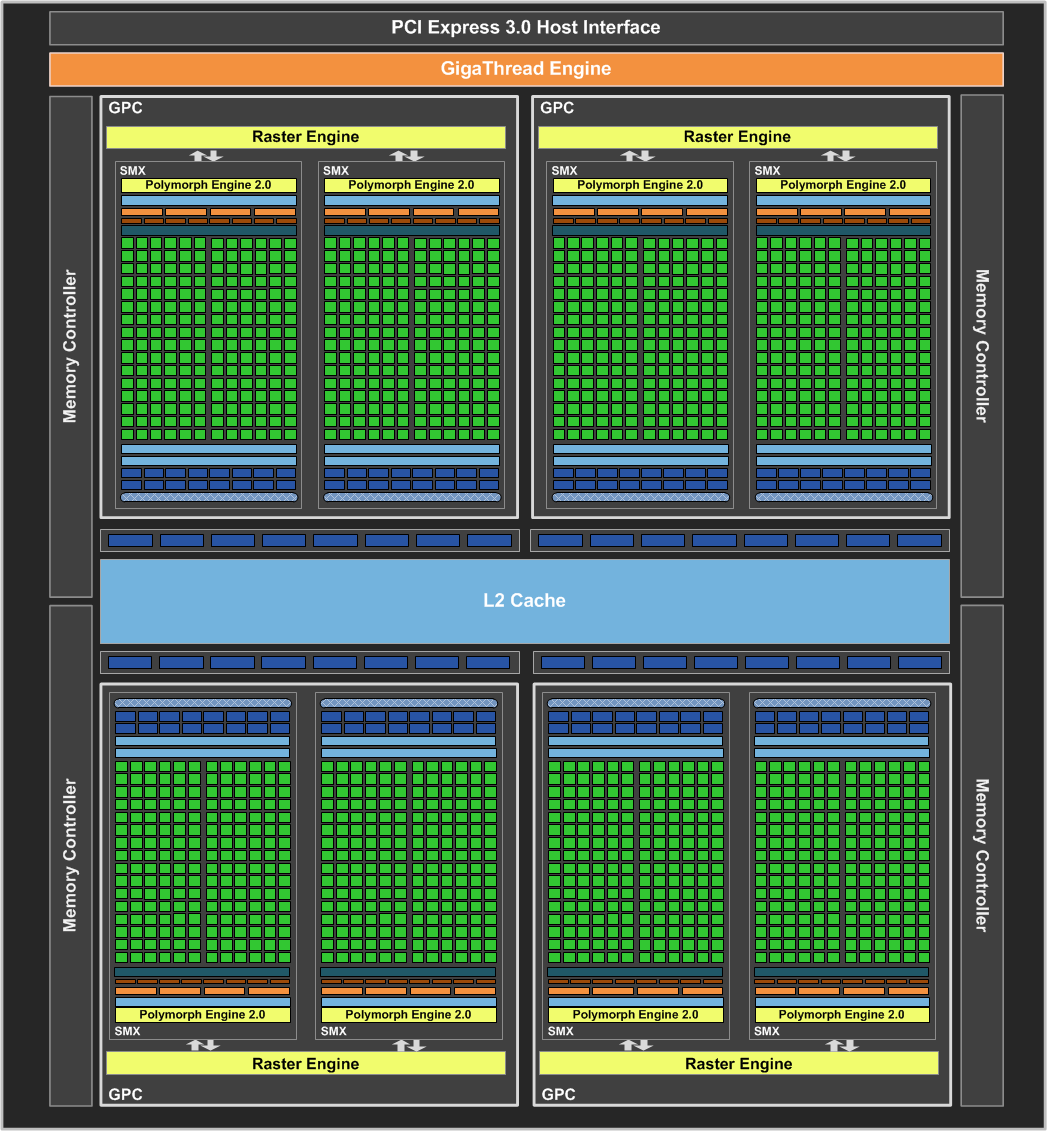
\includegraphics[scale=0.4]{images/kepler-overview.png}
\caption{Architektura Kepler na przykładzie Geforce GTX 680. Źródło: \cite{gf680}}
\label{gf880}
\end{figure}

Jak wynika to ze schematu \ref{gf880} procesory graficzne w architekturze Kepler
zbudowane są z następujących głównych elementów\cite{gf680}:
\begin{itemize}
\item Procesorów Strumieniowych (Streaming Multiprocessor - SMX)
\item Klastrów Graficznych (Graphics Processing Cluster - GPC)
\item Kontrolerów Pamięci (Memory Controllers)
\end{itemize}

Procesory strumieniowe są najważniejszym elementem procesora graficznego. To one
są najbardziej zaawansowane technologicznie, wykonane z nanometryczną
precyzją i przedmiotem nieustannych modyfikacji. Z reguły opracowanie nowej
serii procesorów graficznych zajmuje inżynierom NVIDIA parę lat - i tak w 2012
swoją premierę miała technologii Kepler, a na początku 2014 Maxwell. NVIDIA z
marketingowych względów nie podaje ilości procesorów strumieniowych obecnych w ich GPU. Zamiast tego
podawana jest ilość rdzeni CUDA dostępnych na całym procesorze graficznym.

Najistotniejszym zagadnieniem przy omawianiu implementacji technologii CUDA jest
zrozumienie fundamentalnej różnicy w budowie pomiędzy procesorem strumieniowym a
CPU. Przedstawia to rysunek \ref{cpugpu}, na którym pokazany jest podział
użytych tranzystorów pomiędzy logiczne moduły procesora.  Wynika z
niego, że procesory strumieniowe posiadają mniejszą ilość pamięci cache oraz
mniej skomplikowane sterowanie wykonywaniem instrukcji niż procesory firmy Intel
czy AMD. Wyróżniają się natomiast większą ilością jednostek
arytmetyczno-logicznych (ALU) dostępnych na układzie scalonym. Sprawia to, że
procesory te są wyspecjalizowane w rozwiązywaniu problemów wymagających dużej
intensywności obliczeniowej mierzonej jako stosunek operacji arytmetycznych do
operacji na pamięci.

\begin{figure}[H]
\centering
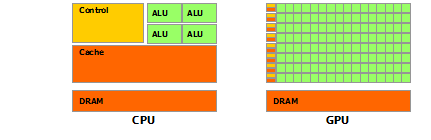
\includegraphics{images/gpu-devotes-more-transistors-to-data-processing.png}
\caption{Podział tranzystorów w architekturze CPU i GPU. Źródło: CUDA C Programming Guide}
\label{cpugpu}
\end{figure}

Kolejnym elementem są klastry graficzne, które służą do grupowania procesorów
strumieniowych oraz pozwalają poprzez ich dodawanie i usuwania na budowanie
odmiennych konfiguracji procesorów graficznych\cite{gf680}. Procesory z większą
ich liczbą, a zatem większą liczbą procesorów strumieniowych, cechować się będą
lepszą wydajnością.

Ostatnim istotnym elementem występującym w procesorach graficznych są kontrolery
pamięci. Zajmują się one pośrednictwem danych pomiędzy pamięcią globalną a
cachem L2 procesorów strumieniowych. Użycie kontrolerów pamięci oznacza, że
pamięć globalna musi być dostarczana przez producenta karty graficznej,
	który musi ją zintegrować z procesorem graficznym. Jest to z
	pewnością elastyczne rozwiązanie, gdyż pozwala produkować sprzęt o różnych
	parametrach, zróżnicowany cenowo. Jednak dla programisty CUDA oznacza to, że
	dostępy do pamięci globalnej są bardzo wolne i
	zawsze powinien on minimalizować serię zapisów i odczytów do pamięci
	globalnej.

Aby przyspieszyć zapis i odczyt z pamięci globalnej procesory graficzne
wyposażone są w cache drugiego poziomu. W Geforce GTX 680 dostępnych
jest jej 512KB . Pamięć ta jest dzielona pomiędzy 4 kontrolery, z czego wynika,
	 że każdy kontroler ma do dyspozycji średnio 128KB tej pamięci. Cache L2
	 jest transparentny dla programistów CUDA i używany jest tylko przez sprzęt
	 w czasie odczytów/zapisu z pamięci globalnej.

\begin{figure}[H]
\centering
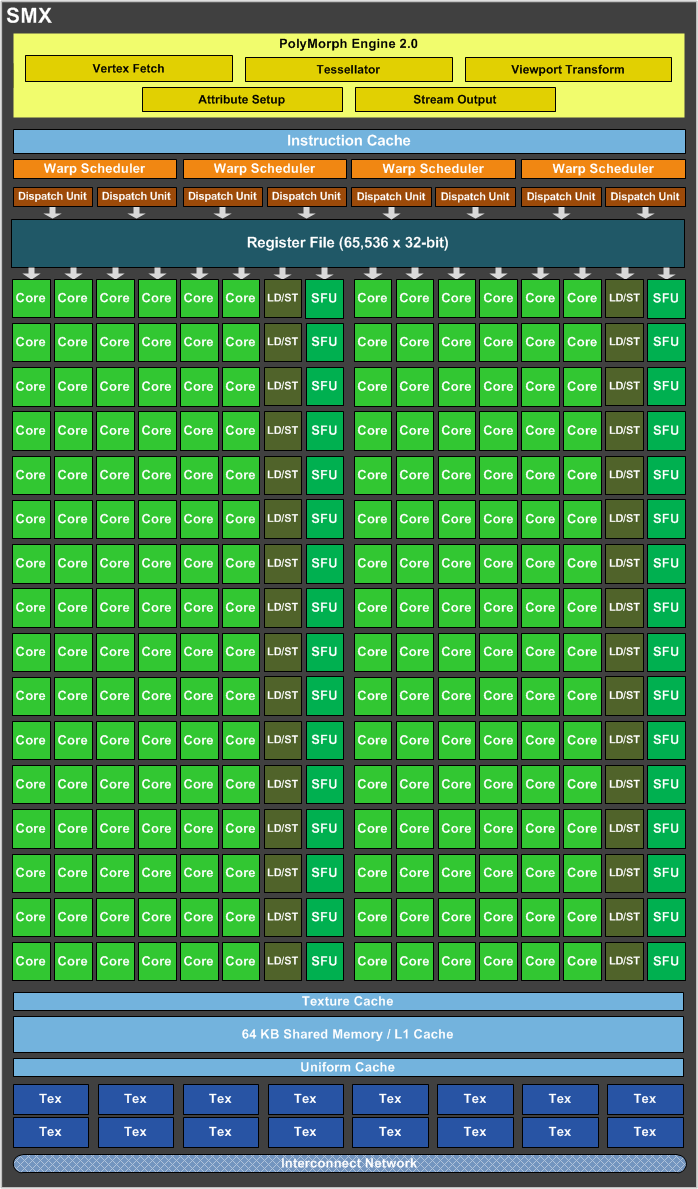
\includegraphics[scale=0.4]{images/kepler-SMX-overview.png}
\caption{Schemat procesora strumieniowego w architektura Kepler. Źródło: \cite{gf680}}
\label{hier2}
\end{figure}

Najważniejszym elementem procesora graficznego jest procesor strumieniowy.
Jego schemat przedstawiony jest na rysunku \ref{hier2}. Do głównych komponentów
procesora strumieniowego, które będą omawiane w tym rozdziale należą:

\begin{itemize}
\item CUDA Core
\item Loading/Storage Unit (LD/ST)
\item Special Function Unit (SFU)
\item Shared Memory / L1 Cache
\item Texture Cache
\item Uniform Cache
\item Warp Scheduler
\end{itemize}

Elementem szczególnego  zainteresowania na powyższym schemacie są rdzenie CUDA
(CUDA cores) oznaczone kolorem zielonym. To one wg NVIDIA głównie decydują o
wydajności danego procesora graficznego. NVIDIA nie podaje ścisłej definicji
czym jest rdzeń CUDA, jednak mogą wg mnie być postrzegane jako procesory będące w
stanie wykonać instrukcje programu CUDA. Posiada jednostki do operacji
na liczbach zmiennoprzecinkowych (FPU) oraz całkowitych (INT Unit).

Loading/Storage Unit są komponentem odpowiedzialnych za czytanie i zapis do
pamięci globalej. Będą one przedmiotem zainteresowania następnych podrozdziałów.

Special Function Unit jest komponentem implementujący sprzętowo pewne znane
operacje na liczbach zmiennoprzecinkowych. Przykładami tych operacji jest
obliczanie przybliżonych wartości funkcji sinus czy cosinus.

Shared Memory / L1 cache jest pamięcią używaną albo do współdzielenia danych
pomiędzy wątkami albo do cachowania danych pochodzących z pamięci L2.

Texture Cache jest specjalnym rodzajem pamięci dedykowanym do obsługi tekstur.
Zasadniczą różnicą pomiędzy nią a zwykłą pamięcią cache jest zastosowanie
zoptymalizowanego algorytmu wczytywania danych. Zamiast operować na fragmencie
pamięci jak na ciągłym obszarze, traktuje on ją jak tablicę dwuwymiarową. W
momencie nie znalezienia potrzebnych danych w cachu (tzw. cache miss'a) w
tablicy na pozycji (x,y), wczytywane są też dane sąsiadujące z nim w rozumieniu
odległości w 2D. Taki algorytm redukuje znacznie ilość cache missów gdy
odwołania do danych przejawiają przestrzenny charakter, jaki ma miejsce w
przypadku renderowania tekstur. Z punktu widzenia programisty CUDA Texture Cache może być
wykorzystany gdy posiadamy ten sam charakter danych lub też gdy zwyczajnie nie
jesteśmy w stanie przewidzieć w jaki sposób będziemy odwoływać się do danych.

Uniform Cache jest w modelu CUDA wykorzystywany do implementacji pamięci
stałej. Jest ona szczególnie szybka w momencie gdy wszystkie wątki odwołują się
do tej samej komórki pamięci w cachu.

\subsection{Warp}

Współbieżne wykonywanie dużej liczby zadań możliwe jest dzięki implementacji
w procesorach graficznych architektury SIMT (Single Intruction Multiple Thread), która
przypomina architekturę SIMD używaną w współczesnych procesorach. W
odróżnieniu od SIMD, który udostępnia tylko możliwość równoległego wykonania danej
operacji na wektorze danych, SIMT umożliwia równoległe wykonywanie wielu
niezależnych wątków. Zaletą wykonywania wątków, zamiast elementarnych operacji jest większa
elastyczność w sterowaniu przepływem programu.

W modelu CUDA zakłada się, że wszystkie wątki w ramach jednego bloku wykonywane
są równolegle. W rzeczywistości jednak procesor graficzny potrafi współbieżnie
wykonywać instrukcje jedynie dla grup wątków zwanych w nomenklaturze CUDA
warpem.  Liczba wątków wchodzących w skład jednego warpa, dla wszystkich
stworzonych do dziś architektur procesorów graficznych NVIDIA, jest stała i
wynosi 32. Z punktu widzenia programisty fakt wykonywania tylko części wątków na
raz może być całkowicie zignorowany, jednak jest istotny do lepszego zrozumienia
działania technologii CUDA i dokonywania zaawansowanych optymalizacji na stworzonym
kodzie \cite{kepler}.

W czasie wykonywania kernela CUDA, każdy blok zostaje wpierw podzielony na
odpowiednią liczbę warpów, a następnie zlecony do wykonania przez jednostkę
procesora strumieniowego zwaną warp schedulerem. To warp scheduler decyduje, który warp
jest w stanie wykonać instrukcję w następnym cyklu zegara. W architekturze
Kepler wszystkie warpy, przydzielone do danego procesora strumieniowego,
zostają rozdystrybuowane pomiędzy 4 dostępne warp schedulery. Te następnie w
każdym cyklu emisji instrukcji są w stanie wykonać po jednej instrukcji na
dwóch zarządzanych przez nie warpach. Oznacza to ostatecznie, że Geforce GTX 680
jest w stanie na każdym procesorze strumieniowym sprzętowo wykonywać maksymalnie 8 * 32 =
256 wątków, co ostatecznie daje krańcową liczbę 2048 wątków dla całego procesora
graficznego.

Możliwość wykonania tylko jednej instrukcji dla danego warpu ma istotnie
konsekwencje. Aby wykonać program, którego następna instrukcja
zależy od danych, NVIDIA wprowadziła możliwość nadawania wątkom jednego z dwóch stanów -
aktywnego oraz pasywnego. Stan aktywny oznacza, że następna instrukcja wątku
zostanie wykonana w następnym cyklu zegara, a pasywny - że egzekucja instrukcji
zostaje w następnym cyklu zawieszona.

W przypadku gdy kod programu danego warpu zawiera tzw. conditional branching,
  czyli zawiera warunek postaci \texttt{if X {...} else {...}}, to najpierw
  zastaną wykonane na 32 wątkach instrukcje programu pierwszej części wyrażenia,
  z oznaczeniem jako pasywnych tych wątków dla których wartość \texttt{X} jest
  nieprawdziwa. Następnie druga strona wyrażenia zostanie wykonana na 32 wątkach
  w analogiczny sposób. Implikacją działania warp schedulera jest fakt, że
  dopiero po wykonaniu obu stron rozgałęzienia programu następne instrukcje mogą
  być wykonane. 
  
Ważne jest zatem aby unikać branchingu w kodzie kerneli CUDA, a
najbardziej sytuacji w których jeden wątek wykonywać będzie długą pętlę, przez
co spowoduje zawieszenie reszty wątków w danym warpie.

\subsection{Dostęp do pamięci}

\begin{figure}[ht]
\centering
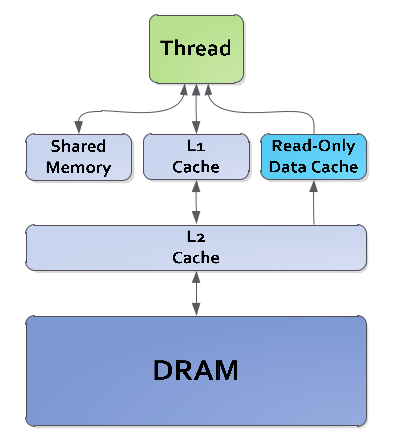
\includegraphics[scale=0.4]{images/memory-hierarchy2.png}
\caption{Hierarchia pamięci w architekturze Kepler: \cite{kepler}}
\label{hierarchiaKepler}
\end{figure}

Wymieniony wcześniej Loading/Storage Unit jest komponentem służącym do odczytów
i zapisów do pamięci globalnej. Każdy dostęp do pamięci globalnej wykonany przez
procesor strumieniowy odbywa się za jego pośrednictwem. Istotną kwestią związaną
z działaniem jednostek LD/ST jest fakt, że dokonują one wczytywania pamięci w
blokach, nazywanych transakcjami. Ilość bajtów wczytanych w jednej transakcji
zależy od architektury urządzenia i dla architektury Kepler wynosi 32, 64 lub
128 bajtów \cite{Nvi11b}. Transakcje dodatkowo muszę być też "wyrównane" (memory
		aligned) tzn. adres początkowy bloku transakcji musi być wielokrotnością
128 bajtów \cite{Nvi11b}.

Wczytanie z pamięci danych, które nie są są "wyrównane", ma negatywny wpływ na
wydajność programu CUDA.  Powyższe założenia dobrze zobrazować przykładem.
Załóżmy, że mamy grupę 32 wątków tworzących warp, które odwołują się do pamięci
globalnej. Jeżeli każdy z nich wczytuje 4 bajty to zakładając, że dane
zaczynają się w pamięci adresem będącym wielokrotnością 128 bajtów, wczytanie
danych odbywa się dokładnie w jednej transakcji o wielkości 128 bajtów. Jest to
optymalna sytuacja minimalizująca użycie jednostek LD/ST procesora graficznego.

Przyjmijmy oznaczenia wywodzące się ze składni języka C. Dane globalne mieszczą się w
tablicy $A[N]$, która jest "wyrównana" do 128 bajtów, a odwołanie do
i-tej komórki tablicy zapiszmy jako $A[i]$. W przypadku, gdy odwołanie następuje
z pewnym przesunięciem $t = 1$, które zapiszemy jako $A[i + 1]$, wczytanie danych
nie może już zostać zrealizowane w jednej transakcji. Dzieje się tak dlatego, że
pierwsza transakcja zostanie i tak zrealizowana od adresu $A[0]$, jednak element
$A[32]$ nie będzie się już w niej zawierał. Dlatego będzie niezbędna będzie
dodatkowa transakcja tylko po to aby wczytać element $A[32]$. Ma to wpływ na
wydajność całego programu CUDA, ponieważ zamiast jednej jednostki LD/ST używane
są dwie dla tej samej grupy wątków. 

Dowodem tego jest wykres \ref{hier2}, na którym pokazano
zależność między wartością przesunięcia a przepustowością.

Przepustowość określa ilości danych, która może zostać przetworzona na
procesorze graficznym w czasie jednej sekundy. W analizowanym przykładzie
wartość przepustowości została obliczona jako czas wywołania kernela CUDA dla
4MB danych. Implementacja kernala zawierała wczytanie wartości z pamięci
globalnej, jej inkrementację oraz ponowny zapis do pamięci globalnej. Dane
empiryczne potwierdzają tezę, że minimalizacja użytych transakcji ma wpływ na
zwiększenie przepustowości programu CUDA. I tak najlepsze rezultaty otrzymujemy
dla $t = 0$ oraz $t = 32$, gdzie $A[32]$ wskazuje na początek następnego
"wyrównanego" bloku pamięci.

\begin{figure}[H]
\centering
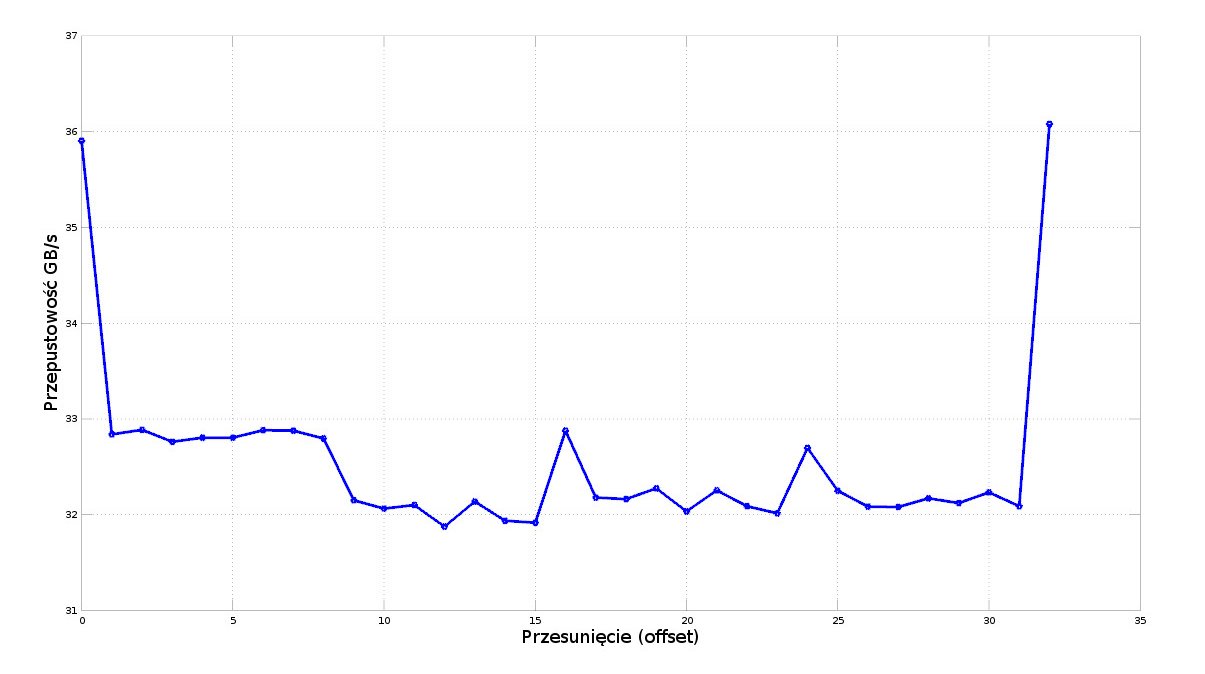
\includegraphics[scale=0.4]{images/gf660_offset.png}
\caption{Pomiar przepustowości Geforce 660M. Źródło: opracowanie własne na
	podstawie \cite{memperf}}
\label{hier2}
\end{figure}

Warto dodać, że teoretyczny spadek wydajności jest realtywnie
mały - z 36 GB/s do 32 GB/s dla Geforca 660M. Ciekawa jest również obserwacja
teoretycznej przepustowości dla innych wartości przesunięcia $t$. Okazuje się,
			 że nie jest ona stała co sugerowałoby założenie o dwóch dokonywanych
			 transakcjach dla każdej grupy wątków. W rzeczywistości
			 kompilator/sterownik dokonuje dodatkowych optymalizacji w
			 zależności od tego do którego niewyrównanego elementu w pamięci staramy się
			 odwołać. Niezależnie jednak od użytych optymalizacji, developer aplikacji CUDA
			 powinien pamiętać, żeby należy wczytywać dane z "wyrównanych"
			 fragmentów pamięci.

Dużo większy wpływ na spadek wydajności ma wczytywanie danych nie ułożonych gęsto w
pamięci, a rozdzielonych stałymi odstępami liczonymi w bajtach. Ma to np. miejsce w przypadku gdy
dane aplikacji CUDA reprezentowane są jako tablica struktur (Array of Struct, AOS), a deweloper
odwołuje w kernelu tylko do jednego pola tej struktury. Efekt zwiększania odstępów
między kolejnymi polami struktur przedstawia wykres \ref{hier}. Rozwiązaniem tego
problemu może być reprezentacja danych jako struktury tablic (Struct of Array,
		SOA).

\begin{figure}[H]
\centering
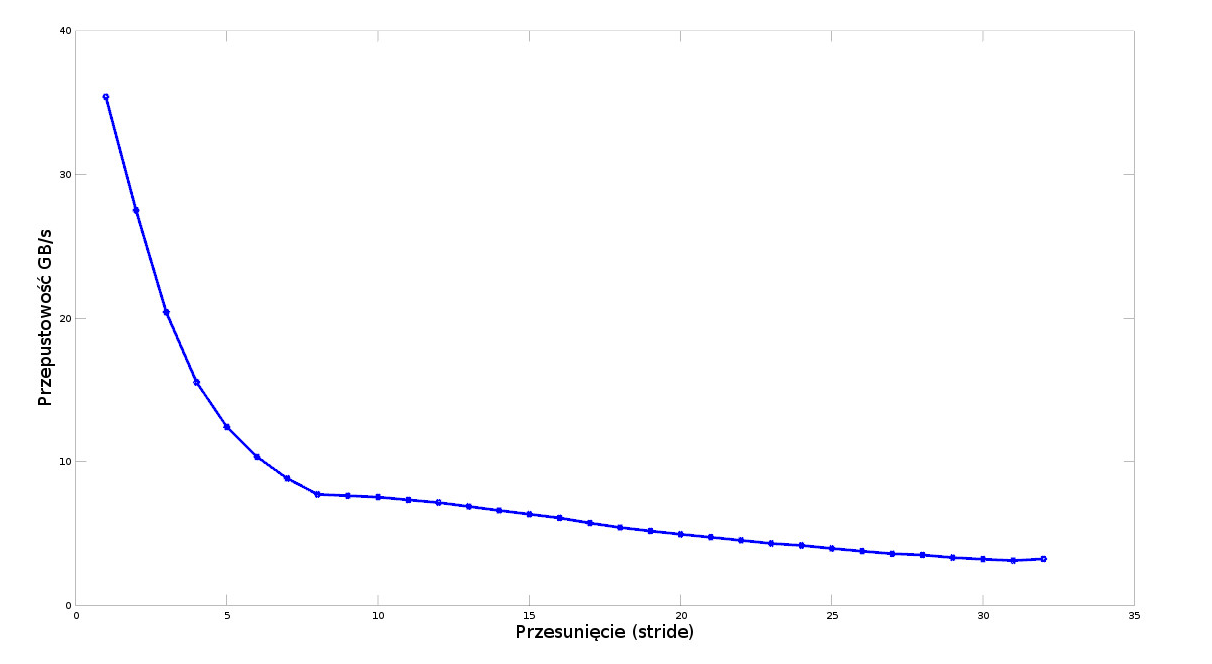
\includegraphics[scale=0.4]{images/gf660_stride.png}
\caption{Pomiar przepustowości Geforce 660M. Źródło: opracowanie własne na
	podstawie \cite{memperf}}
\label{hier}
\end{figure}
